%\documentclass{nature}
\documentclass[12pt, letterpaper]{article}
\usepackage{graphicx}
%\usepackage{hyperref}
\usepackage{xcolor}
\usepackage[capposition=top]{floatrow}
\usepackage[center]{caption}
\usepackage[flushleft]{threeparttable}
%\usepackage[superscript,biblabel]{cite}

%\bibliographystyle{naturemag}
%\usepackage{apacite}
\usepackage[style=nature]{biblatex}
%\usepackage[backend=biber,style=numeric,sorting=none]{biblatex}
%\usepackage[backend=biber]{biblatex}

\definecolor{green}{rgb}{0,1,0}
\newcommand{\NS}[1] {{\textcolor{green}{#1}}}

%I will need to fix the references
\addbibresource{football_refs.bib}
\begin{document}
\title{Reported cases of alcohol-related domestic abuse increase following the victory of the England national football team}

%title: I am using the word "reported" to highlight the issue of underreporting, and I am also cautious about not claiming causal effects, but emphasize that the increase starts when the match starts

\author{Anna Trendl}
\textbf{Letter}:
A Letter is an important research study of high quality and general interest to human behaviour researchers.  The text is approximately 5,000 words, including the introductory paragraph, but excluding references and figure legends. Letters should have no more than 4 display items (figures and/or tables). As a guideline, Letters contain approximately 30 references (excluding those cited exclusively in Methods). This format begins with a title of, at most, 90 characters (including spaces), followed by an introductory paragraph (not abstract) of approximately 200 words, summarizing the background, rationale, main results (introduced by "Here we show" or some equivalent phrase) and implications of the study. This paragraph should be fully referenced and should be considered part of the main text, so that any subsequent introductory material avoids too much redundancy with the introductory paragraph. Letters are not divided by headings, except for the Methods heading.

Letters include received/accepted dates and may be accompanied by supplementary information. Letters are peer reviewed.


\maketitle

\NS{Neil crappy abstract: When England wins or loses a football match, we use WMP data to show that there is a 60\% spike in domestic abuse cases.  We only see the patterns for wins and losses not draws, and only see the increase for domestic abuse cases involving alcohol. Indeed the spike is unique to male on female intimate partner domestic abuse, and we don't see it for other types of incident (e.g., antisocial behaviour).}

\section{Introductory para (200 words approx)}

Understanding the factors that contribute to the occurrence of violence in family and intimate partner relationships is key for designing effective interventions to protect victims. Previous research has suggested that national football (soccer) tournaments increase the number of reported domestic abuse cases in England\autocite{Kirby2014, Brimicombe2012}. While hypothesized to be a significant factor, previous quantitative research has not explored the role of alcohol in this relationship. Using crime data from the third largest police force in England, serving a population of 2.9 million\autocite{populationfigure}, we find that the number of reported alcohol-related domestic abuse cases increases by 62\% following an England victory in a national football tournament (World Cup, European Championship). This effect is driven by a 72\% increase in male to female alcohol-related cases, is absent from male to male, female to male, and female to female domestic abuse cases, and is not present in other types of criminal behaviours, such as public order offences, other violent, or property-related offences, \NS{or hate crimes}. A three-hour analysis reveals that the increase starts in the three-hour period of the match, peaks in the three hours after the victory, and gradually declines to its baseline level in the 24 hours following the match. The abuse that occurs is not characteristically different from domestic abuse cases occurring on non-match days, apart from the stronger association with alcohol. \NS{Whatever the football does, it only does it to men, only when they are drunk, and only affects their behaviour towards the females they know.}

\section{Long intro}

"If England gets beaten, so will she" - read the poster as part of the "The Not-So-Beautiful-Game" awareness campaign launched by the National Centre for Domestic Violence in the wake of the 2018 FIFA World Cup \autocite{NCDV}. While the link betwen sport events and domestic abuse has been the focus of a number of smaller studies\autocite{Williams2014}, large-scale quantitative investigations of this relationship are relatively scarce. The most extensive study in the topic found that an unexpected loss of the local National Football League (NFL) team resulted in a 10\% increase in the rate of reported male to female intimate partner violence (IPV) in the US\autocite{Card2011}. 

In England, most studies have focused on the link between football (soccer) and domestic abuse. Football's history is inextricably linked to England, and is by far the most popular sport in the country \autocite{Parry2014}, with the 2018 World Cup attracting record number of viewers \autocite{BBC}. In 2012, a small, exploratory study investigated the effect of the 2010 World Cup on domestic abuse, using data from 33 out of 39 police forces in England\autocite{Brimicombe2012}. Using a control period from 2009, the study found that rates of reported domestic abuse increased significantly when England lost or won (about 33-35\%), but did not change on days then they draw. A more comprehensive investigation, using daily counts of domestic abuse in Lancashire from the 2002, 2006 and 2010 World Cup, found a 38\% increase in the number of reported domestic violence cases when the England team lost, and a 26\% increase when they won or drew\autocite{Kirby2014}. These estimates had been widely discussed in the British media before the 2018 World Cup, and the figures were also quoted on the posters in the Not-so Beautiful Game Campaign. While domestic abuse is predominantly understood as a pattern of ongoing behaviour, involving a series of occurrences, rather than a one-off incident triggered by football \autocite{Brooks-Hay2018}, these studies, and other qualitative investigations\autocite{Swallow} nevertheless suggest that national football tournaments can create an environment for abusers that is conducive to domestic abuse.

Why would national football tournaments, such as the World Cup or the European Championship precipitate domestic abuse? England's participation in these tournaments are times of heightened patriotic emotions and a strengthened sense of "Englishness", fuelled by media narratives that often use war references and a "us vs. them" rhetoric to generate and represent an English national identity\autocite{Vincent2014}.  Previous qualtitatve research has suggested that televised contact sports can serve as vehicle for the male sports fan to redefine and express his masculinity in a way that allows dominance, control, and can ultimately manifest in the perpetration of domestic abuse, given susceptibility to such behaviours\autocite{Sabo,Swallow}. We speculate that this observation is especially pertinent in the context of England's participation in national tournaments, owing to the popularity of the sport in the country, the associated media attention, and the heightened sense of national consciousness.

Qualitative investigations suggest that alcohol can be a significant factor in the link between football and domestic abuse. Alcohol has a strong association with domestic abuse, those with alcohol-problems are more likely to be perpetrators, and when alcohol is involved, there is evidence that the violence might result in more serious injuries \autocite{Peralta2010}. However, it is generally understood that the role of alcohol should be considered in the context of a range of social, biological and pyschological factors, and that alcohol is never the direct cause of domestic abuse \autocite{Javaid2015,Peralta2010}. One explanation for the co-occurrence of domestic abuse and alcohol suggest that for some men, drinking and violence plays an instrumental role in the construction and expression of masculinity, especially when the problem of masculine deficiency is present (e.g., by unemployment)\autocite{Peralta2010}. 

In the US, the relationship between unexpected NFL losses and IPV did not depend on alcohol-involvement in the incident\autocite{Card2011}. While England-based quantitative studies did not look at the role of alcohol in particular, given the strong association between drinking culture and football in England\autocite{Dixon2014}, a relationship continuously reinforced by the marketing practices of the alcohol industry\autocite{Gornall2014}, we hypothesize that alcohol might play an important role in the relationship between national football tournaments and domestic abuse.

To explore this hypothesis, we investigate whether the number of reported domestic abuse cases recorded by the West Midland Police in England between 2010 and 2018 increase on days when the England national team plays in the World Cup or the European Championship, and whether the effect, if any, is affected by alcohol-involvement. We also consider whether the result of the match alters the relationship, as previous research suggested that the effect is heightened when England loses\autocite{Kirby2014}. Our unique dataset also allows us to investigate various aspects of the link between football tournaments and domestic abuse.


\newpage

\subsection{Data description}

Our dataset comprises all crimes and specific types of incidents (such as domestic abuse) that have been reported to the West Midlands Police (the third largest police force in England\autocite{Homeoffice}, serving an estimated 2.9 million people in 2017\autocite{populationfigure}) in the period between 2010 and 2018\footnote{The first half of 2017 has been excluded due to missing data.}. The number of reported domestic abuse cases is the sum of crimes that have a domestic abuse marker, and all domestic abuse incidents. Crimes that have a domestic abuse marker indicate cases of domestic abuse that meet the criteria for notifiable offences in the UK, whereas domestic abuse incidents refer to cases that do not qualify as a crime. For each record in this dataset, we have information about the time and location of the incident or crime, and the gender and age of the offender and victim. We can also identify repeat offenders and victims by their unique person identifier. Domestic abuse cases comprise about 31\% of all recorded crimes and incidents in the dataset, and about 23\% of all domestic abuse cases are alcohol-related. \textcolor{red}{Sentence about daily rate and how it compares to previous studies}. There were three World Cups (2010, 2014, 2018) and two European Championships (2012, 2016) in the period covered by our dataset. Both tournaments take place in the months of June and July.

In the UK, the term "domestic abuse" refers to a wide range of behaviours, from physical and sexual violence to psychological, emotional, financial abuse, threatening behaviour, stalking and harassment either within a family or an intimate relationship\autocite{ONS}. Recent changes to the definition introduced the concept of coercive control, which recognises domestic abuse as a pattern of incidents, which can include any of the above behaviours. Previous research have mostly focused on IPV, which the largest subcategory of domestic abuse. 




\textcolor{red}{Card \& Dahl find a 10\% increase in male to female violence, in their dataset, daily prevalence of DA is 1.28 per 100,000 population,10\% increase is 0.128 increase in daily rate, our rates are quite variable (also something happens in 2012), but the average is 0.72, 60\% increase is 0.43 increase in daily rate}
 
\textcolor{red}{this table is just for illustration}

\begin{table}[ht]
\centering
\begin{tabular}{rrlrrrr}
  \hline
 & year & Alcohol & No\_days & DA\_cases & Population & Rate \\ 
  \hline
1 & 2010 & No & 365 & 23332 & 2711938.00 & 2.36 \\ 
  2 & 2010 & Yes & 365 & 3978 & 2711938.00 & 0.40 \\ 
  3 & 2011 & No & 365 & 20887 & 2739733.00 & 2.09 \\ 
  4 & 2011 & Yes & 364 & 3490 & 2739733.00 & 0.35 \\ 
  5 & 2012 & No & 366 & 15789 & 2761887.00 & 1.56 \\ 
  6 & 2012 & Yes & 364 & 3611 & 2761887.00 & 0.36 \\ 
  7 & 2013 & No & 365 & 22422 & 2781753.00 & 2.21 \\ 
  8 & 2013 & Yes & 365 & 7732 & 2781753.00 & 0.76 \\ 
  9 & 2014 & No & 365 & 27758 & 2805891.00 & 2.71 \\ 
  10 & 2014 & Yes & 365 & 10005 & 2805891.00 & 0.98 \\ 
  11 & 2015 & No & 365 & 30225 & 2834490.00 & 2.92 \\ 
  12 & 2015 & Yes & 365 & 10931 & 2834490.00 & 1.06 \\ 
  13 & 2016 & No & 366 & 31499 & 2870551.00 & 3.00 \\ 
  14 & 2016 & Yes & 366 & 11005 & 2870551.00 & 1.05 \\ 
  15 & 2017 & No & 289 & 12909 & 2897303.00 & 1.54 \\ 
  16 & 2017 & Yes & 187 & 4232 & 2897303.00 & 0.78 \\ 
  17 & 2018 & Yes & 310 & 9109 &  &  \\ 
  18 & 2018 & No & 310 & 28479 &  &  \\ 
   \hline
\end{tabular}
\end{table}

Our dataset contains all cases of domestic abuse reported to the police, but the vast majority of all domestic abuse incidents in fact never get reported (according to the Crime Survey of England and Wales, only 17\% of all domestic abuse victims reported the abuse to the police between April, 2017 and March, 2018\autocite{ONS}). This substantial reporting bias, and its potential correlation with other contextual factors warrants a careful interpretation of the estimates from any quantitative study, and highlights the importance of utilising a mixed methods approach to explore the factors contributing to domestic abuse. 

\clearpage


\section{Results}

In the following regressions, each observation is a day in the period between 2010 and 2018, and the outcome variable is the number of domestic abuse cases reported to have been perpetrated on that day. To investigate whether national football tournaments affect the number of reported abuse cases, we classify each day in our dataset as either a day on which England won (England win), lost (England lost) or drew (England draw), a day after an England match day (After England), any other day during the tournament (Tournament on), or any other day during the rest of the year (Nonmatch day). 

We first explore whether adding this day classification variable to a baseline model results in an improved model fit. The results in Table \ref{specifications} show that adding our day classification variable to a baseline model with alcohol and a set of control variables reduces AIC (see column 1 and 2), and that an England victory increases the number of reported abuse cases by 21\%. Including a interaction term between alcohol and type of day (see column 3) further improves the model, and indicates a 61\% increase in alcohol-related domestic abuse incidents on days when the England national team wins. 



\begin{table*}
\centering
\scalebox{0.9}{
  \begin{threeparttable}
  \caption{Number of reported domestic abuse incidents by alcohol involvement and type of day} 
  \label{specifications}
\begin{tabular}{@{\extracolsep{5pt}}lccc} 
\\[-1.8ex]\hline 
\hline \\[-1.8ex] 
 & \multicolumn{3}{c}{\textit{Dependent variable:}} \\ 
  & \multicolumn{3}{c}{Number of domestic abuse cases per day} \\ 
\cline{2-4} 
%\\[-1.8ex] & \multicolumn{3}{c}{N} \\ 
% & All & Male to Male & Male to Female \\ 
\\[-1.8ex] & (1) & (2) & (3)\\ 
\hline \\[-1.8ex] 
 Alcohol & $-$0.720$^{***}$ & $-$0.720$^{***}$ & $-$0.721$^{***}$ \\ 
  & (0.008) & (0.008) & (0.008) \\ 
  Tournament on &  & $-$0.013 & 0.013 \\ 
  &  & (0.026) & (0.032) \\ 
  England win &  & 0.210$^{***}$ & $-$0.037 \\ 
  &  & (0.073) & (0.097) \\ 
  England draw &  & 0.022 & 0.047 \\ 
  &  & (0.087) & (0.112) \\ 
  England lost &  & 0.078 & $-$0.016 \\ 
  &  & (0.073) & (0.095) \\ 
  After England &  & 0.095$^{**}$ & 0.073 \\ 
  &  & (0.046) & (0.059) \\ 
  Alcohol:Tournament on &  &  & $-$0.065 \\ 
  &  &  & (0.046) \\ 
  Alcohol:England win &  &  & 0.612$^{***}$ \\ 
  &  &  & (0.144) \\ 
  Alcohol:England draw &  &  & $-$0.060 \\ 
  &  &  & (0.175) \\ 
  Alcohol:England lost &  &  & 0.227 \\ 
  &  &  & (0.143) \\ 
  Alcohol:After England &  &  & 0.049 \\ 
  &  &  & (0.089) \\ 
 \hline \\[-1.8ex] 
Observations & 6,034 & 6,034 & 6,034 \\ 
Log Likelihood & $-$23,017.270 & $-$23,011.260 & $-$23,003.430 \\ 
%$\theta$ & 16.869$^{***}$  (0.466) & 16.911$^{***}$  (0.468) & 16.979$^{***}$  (0.470) \\ 
Akaike Inf. Crit. & 46,092.530 & 46,090.530 & 46,084.860 \\ 
\hline 
\hline \\[-1.8ex] 
%\textit{Note:}  & \multicolumn{3}{r}{$^{*}$p$<$0.1; $^{**}$p$<$0.05; $^{***}$p$<$0.01} \\ 
\end{tabular}  
\begin{tablenotes}
      \item[a] \textit{$^{*}$p$<$0.1; $^{**}$p$<$0.05; $^{***}$p$<$0.01}
      \item[b] \textit{Estimates are from a series of negative binomial regressions (based on tests of overdispersion)  with year, month, day of week, Christmas, New Year's eve controls; standard errors in parentheses}
    \end{tablenotes}
\end{threeparttable} }
\end{table*}


We can also investigate whether the effect varies by the gender of the perpetrator and the victim. Previous qualitative research has suggested that the link between football and domestic abuse is a result of violent expression of masculinity, where heavy drinking is also often present\autocite{Sabo}. If this was the case, we would expect football and alcohol to only affect reported numbers of male-perpetrated domestic abuse. 


The first column of Table \ref{gender_regression} shows the result for all reported domestic abuse cases, and the remaining four columns show the result for different offender-victim gender groups. The results show that for all cases of domestic abuse, we see a 61\%, 95\% CI [22--113] increase in alcohol-related cases on days when England won, compared to non-match days. This increase is driven by Male to Female abuse (which comprises about 80\% of all domestic abuse cases in our data), where the increase is 71\%, 95\% CI [28--129]. These results suggest that football and alcohol only makes men more violent, and only towards women. 

\begin{table*}
\centering
\scalebox{0.9}{
  \begin{threeparttable}
  \caption{Number of reported domestic abuse incidents by type of day, alcohol involvement, and gender of perpetrator and victim} 
  \label{gender_regression}
\begin{tabular}{@{\extracolsep{5pt}}lccccc} 
\\[-1.8ex]\hline 
\hline \\[-1.8ex] 
 & \multicolumn{5}{c}{\textit{Dependent variable:}} \\ 
  & \multicolumn{5}{c}{Number of domestic abuse cases per day} \\ 
\cline{2-6} 
\\[-1.8ex] &  & \multicolumn{4}{c}{} \\ 
 & All & Male to & Male to & Female to & Female to \\ 
 & Cases & Male & Female & Female & Male \\ 
\\[-1.8ex] & (1) & (2) & (3) & (4) & (5)\\ 
\hline \\[-1.8ex] 
Tournament on & 0.013 & $-$0.021 & 0.021 & 0.043 & $-$0.122$^{*}$ \\ 
  & (0.032) & (0.061) & (0.032) & (0.071) & (0.053) \\ 
  England win & $-$0.037 & $-$0.046 & $-$0.037 & 0.042 & $-$0.141 \\ 
  & (0.097) & (0.175) & (0.099) & (0.199) & (0.150) \\ 
  England draw & 0.047 & 0.083 & 0.035 & 0.063 & 0.057 \\ 
  & (0.112) & (0.205) & (0.114) & (0.232) & (0.184) \\ 
  England lost & $-$0.016 & $-$0.063 & $-$0.009 & $-$0.039 & 0.089 \\ 
  & (0.095) & (0.172) & (0.097) & (0.177) & (0.150) \\ 
  After England & 0.073 & $-$0.025 & 0.075 & 0.172$^{*}$ & 0.019 \\ 
  & (0.059) & (0.108) & (0.060) & (0.117) & (0.090) \\ 
 % Alcohol & $-$0.721$^{***}$ & $-$0.610$^{***}$ & $-$0.733$^{***}$ & $-$0.610$^{***}$ & $-$0.728$^{***}$ \\ 
%  & (0.008) & (0.018) & (0.008) & (0.023) & (0.015) \\ 
  Tournament on:Alcohol & $-$0.065 & $-$0.147 & $-$0.055 & $-$0.080 & $-$0.048 \\ 
  & (0.046) & (0.108) & (0.048) & (0.139) & (0.087) \\ 
  England win:Alcohol & 0.612$^{***}$ & 0.267 & 0.714$^{***}$ & 0.226 & 0.458 \\ 
  & (0.144) & (0.293) & (0.148) & (0.358) & (0.246) \\ 
  England draw:Alcohol & $-$0.060 & $-$0.305 & 0.010 & $-$0.034 & $-$0.500 \\ 
  & (0.175) & (0.417) & (0.181) & (0.627) & (0.325) \\ 
  England lost:Alcohol & 0.227 & 0.293 & 0.195 & 0.297 & 0.032 \\ 
  & (0.143) & (0.286) & (0.150) & (0.356) & (0.243) \\ 
  After England:Alcohol & 0.049 & 0.152 & 0.078 & $-$0.197 & $-$0.006 \\ 
  & (0.089) & (0.183) & (0.092) & (0.234) & (0.162) \\ 
  \hline \\[-1.8ex] 
Observations & 6,034 & 6,034 & 6,034 & 6,034 & 6,034 \\ 
%Log Likelihood & $-$22,935.480 & $-$10,790.100 & $-$21,788.040 & $-$9,318.764 & $-$12,729.650 \\ 
%$\theta$ & 17.116$^{***}$  (0.475) & 31.912$^{***}$  (6.562) & 17.098$^{***}$  (0.509) & 34.754$^{***}$  (9.990) & 21.271$^{***}$  (2.122) \\ 
%Akaike Inf. Crit. & 45,948.950 & 21,658.200 & 43,654.080 & 18,715.530 & 25,537.310 \\ 
\hline 
\hline \\[-1.8ex] 
%\textit{Note: Negative binomial regressions with year, month, day of week, Christmas, New Year's eve controls}  & \multicolumn{5}{r}{$^{*}$p$<$0.1; $^{**}$p$<$0.05; $^{***}$p$<$0.01} \\ 
\end{tabular} 
\begin{tablenotes}
      \item[a] \textit{$^{*}$p$<$0.1; $^{**}$p$<$0.05; $^{***}$p$<$0.01}
      \item[b] \textit{Estimates are from a series of negative binomial regressions (based on tests of overdispersion)  with year, month, day of week, Christmas, New Year's eve controls; standard errors in parentheses}
    \end{tablenotes}
\end{threeparttable} }
\end{table*}

These findings show both similarities and differences with results from previous research. A similarity is that the increase is only present in male to female abuse cases, lending support to the hypothesis that masculinity construction coupled with alcohol consumption can be key in the link between sports-induced violence and domestic abuse. However, in the US study\autocite{Card2011}, the effect of the match did not depend on alcohol-involvement in the abuse case, and the increase was driven by unexpected losses, whereas our findings suggest that it is a victory that results in the largest increase, and that alcohol plays an instrumental role in the relationship between football and domestic abuse. This discrepancy highlights that the effect on sports-induced emotional cues on domestic abuse are sensitive to the cultural context. 

Based on the pre-match betting odds, all England victories were expected in our dataset, suggesting that in the context of England's participation in national football tournaments, it is living up to the hopes of the fans that has the largest emotional effect, and perhaps results in increased alcohol consumption\autocite{Davies2018}. Previous research has demonstrated how the vicarious experience of watching their team play can increase supporter's testosterone and cortisol levels, even when they expect their team to win, which has been suggested to be an adaptive response to the perceived threat to one's social identity\autocite{VanderMeij2012}.

%In the context of the World Cup, previous research has reported elevated testosterone levels amongst the winning team's supporters\autocite{Bernhardt1998}.

The largest England-based study found that an England loss results in the largest increase (38\%) in domestic abuse, and a win or draw have a slightly smaller effect (26\%)\autocite{Kirby2014}. We find a slightly different pattern (although the difference between the effect of an England win and loss on alcohol-related cases is not significant, see Table \ref{emmeans_results} in the Appendix), in that it is when England wins we find the largest increase in domestic abuse. Upon re-analysing their data by treating wins and draws as two separate variables and adding a month control (see Table \ref{kirbyrep} in the Appendix), we see a more similar effect to ours, where wins result in the largest increase (46\%, 95\% CI [29--65]), followed by losses (33\%, 95\% CI [11--59]), and no effect when England draws (possibly due to the fact that high-stake matches after the group-stage in the tournament cannot result in a draw). Taken together with our findings, these results suggest that the link between football and domestic abuse is mostly driven by victories, and to a lesser extent by losses, and that alcohol plays a key role in this relationship.

\textcolor{red}{difference between the emotional impact of a victory and a loss? why are victories so much more salient? but both are alcohol-related}

Our unique dataset further allows us to explore whether England games have similar effects on other types of criminal behaviours. Specifically, we are interested in how an England match day affects the number of reported public order offences (behaviours that cause offence to the general public), property-related crimes (including burglary, theft and robbery), and other violent crimes (excluding cases of domestic abuse).  Of particular interest is the effect of football on non-domestic violent crimes, since it is possible that alcohol-fuelled violence that follows an England victory is not limited to family relationships.

Table \ref{othertype_regression} shows the result from four regressions, one for each type of criminal behaviour, including domestic abuse. Compared to non-match days, we see more non-alcohol related public order offence cases during the tournament, when England wins, and the day following an England game, potentially a sign of temporal spillover effects from the game. Perhaps surprisingly, we do not see strong differential effects for alcohol-related public order offences. Interestingly, non-domestic and non-alcohol related violent crimes only increase after an England game day, and not on the day of the game. More importantly, the effect of an England win on alcohol-related incidents is clearly unique to domestic abuse, indicating that whatever causes an increase in alcohol-related domestic abuse following an England victory, it does not extend to violence against non-family members. 

\textcolor{red}{For violent offences, a regression on the subset of alcohol-related offences only yield an England win effect. I think it doesn't come out in the regression with interaction because there's also a slight increase in non-alcohol related offences as well.}



\begin{table}[!htbp]
 \centering 
 \scalebox{0.9}{
  \begin{threeparttable}
  \caption{Number of reported cases for each crime type, by type of day, and alcohol involvement} 
  \label{othertype_regression}
\begin{tabular}{@{\extracolsep{5pt}}lcccc} 
\\[-1.8ex]\hline 
\hline \\[-1.8ex] 
 & \multicolumn{4}{c}{\textit{Dependent variable:}} \\ 
\cline{2-5} 
%\\[-1.8ex] & DA\_incidents & Public\_order\_offences & Property\_related & Violence\_Against\_The\_Person \\ 
 & Domestic  & Public Order  & Property- & Other  \\ 
 &  Abuse & Offences & related & Violence  \\ 
\\[-1.8ex] & (1) & (2) & (3) & (4)\\ 
\hline \\[-1.8ex] 
Tournament on & 0.013 & 0.090$^{**}$ & 0.049$^{*}$ & 0.077$^{*}$ \\ 
  & (0.032) & (0.038) & (0.028) & (0.042) \\ 
  England win & $-$0.037 & 0.271$^{**}$ & 0.074 & 0.212 \\ 
  & (0.097) & (0.102) & (0.082) & (0.127) \\ 
  England draw & 0.047 & $-$0.084 & 0.113 & 0.071 \\ 
  & (0.112) & (0.137) & (0.094) & (0.148) \\ 
  England lost & $-$0.016 & 0.059 & $-$0.057 & 0.080 \\ 
  & (0.095) & (0.109) & (0.086) & (0.127) \\ 
  After England & 0.073 & 0.173$^{**}$ & 0.050 & 0.197$^{**}$ \\ 
  & (0.059) & (0.066) & (0.052) & (0.078) \\ 
%  Alcohol & $-$0.721$^{***}$ & $-$0.886$^{***}$ & $-$0.949$^{***}$ & $-$0.798$^{***}$ \\ 
%  & (0.008) & (0.016) & (0.013) & (0.011) \\ 
  Tournament on:Alcohol & $-$0.065 & $-$0.154$^{*}$ & 0.048 & $-$0.091 \\ 
  & (0.046) & (0.094) & (0.071) & (0.062) \\ 
  England win:Alcohol & 0.612$^{***}$ & $-$0.208 & 0.150 & 0.167 \\ 
  & (0.144) & (0.267) & (0.221) & (0.191) \\ 
  England draw:Alcohol & $-$0.060 & 0.419 & $-$0.056 & 0.175 \\ 
  & (0.175) & (0.310) & (0.264) & (0.226) \\ 
  England lost:Alcohol & 0.227 & 0.519$^{*}$ & 0.330 & $-$0.017 \\ 
  & (0.143) & (0.231) & (0.230) & (0.195) \\ 
  After England:Alcohol & 0.049 & 0.065 & 0.085 & $-$0.136 \\ 
  & (0.089) & (0.155) & (0.140) & (0.119) \\ 
 \hline \\[-1.8ex] 
Observations & 6,034 & 6,034 & 6,034 & 6,034 \\ 
%Log Likelihood & $-$23,487.520 & $-$13,718.040 & $-$17,804.140 & $-$22,298.810 \\ 
%$\theta$ & 16.599$^{***}$  (0.447) & 25.212$^{***}$  (1.912) & 29.528$^{***}$  (1.303) & 8.700$^{***}$  (0.228) \\ 
%Akaike Inf. Crit. & 47,053.040 & 27,514.090 & 35,686.280 & 44,675.630 \\ 
%\hline 
%\hline \\[-1.8ex] 
%\textit{Note:}  & \multicolumn{4}{r}{$^{*}$p$<$0.1; $^{**}$p$<$0.05; $^{***}$p$<$0.01} \\ 
\hline 
\hline \\[-1.8ex] 
\end{tabular} 
\begin{tablenotes}
      \item[a] \textit{$^{*}$p$<$0.1; $^{**}$p$<$0.05; $^{***}$p$<$0.01}
      \item[b] \textit{Estimates are from a series of negative binomial regressions (based on tests of overdispersion)  with year, month, day of week, Christmas, New Year's eve controls; standard errors in parentheses}
    \end{tablenotes}
\end{threeparttable} }
\end{table}
Next, we explore the temporal dynamics of the increase in alcohol-related domestic abuse on England match days in more detail. To this end, we divided each day in our dataset into eight three-hour periods, the first one starting at 12am, and used these to identify specific time windows around the time of the match. The exact time of the matches vary considerably (the earliest starting at 1pm, and the latest at 11pm). We first identified the three-hour period of the day into which each match falls. If the start and end time of the match did not fall in the same three-hour period, we chose the three-hour period that covers the larger part of the match (e.g., a 2.5 hour long match starting at 7pm will be assigned to the 6-9pm period and not to the 9pm-12am period). Based on our previous results, we analyse the effect by the result of the match and alcohol-involvement in the case, by running two separate regressions for alcohol and non-alcohol related domestic abuse cases.

Figure \ref{fig:threehours} shows a plot of the coefficients from these regressions, which reveals a stark increase in alcohol-related domestic abuse on days of an England victory, starting in the three hour period of the match, peaking in the three-hour period afterwards, and gradually declining to its original level in the twenty-four hours following the victory. We see a similar pattern, albeit much less pronounced, in alcohol-related domestic abuse on days when England lost. These results strongly suggest that the emotional effect of a win or loss drive the subsequent increase in alcohol-related domestic abuse. It also highlights the possibility that the asymmetric effect of England victories might stem from prolonged post-match celebrations coupled with increased alcohol consumption.


\begin{figure}
\centering
 \caption{The temporal dynamics of the effect}
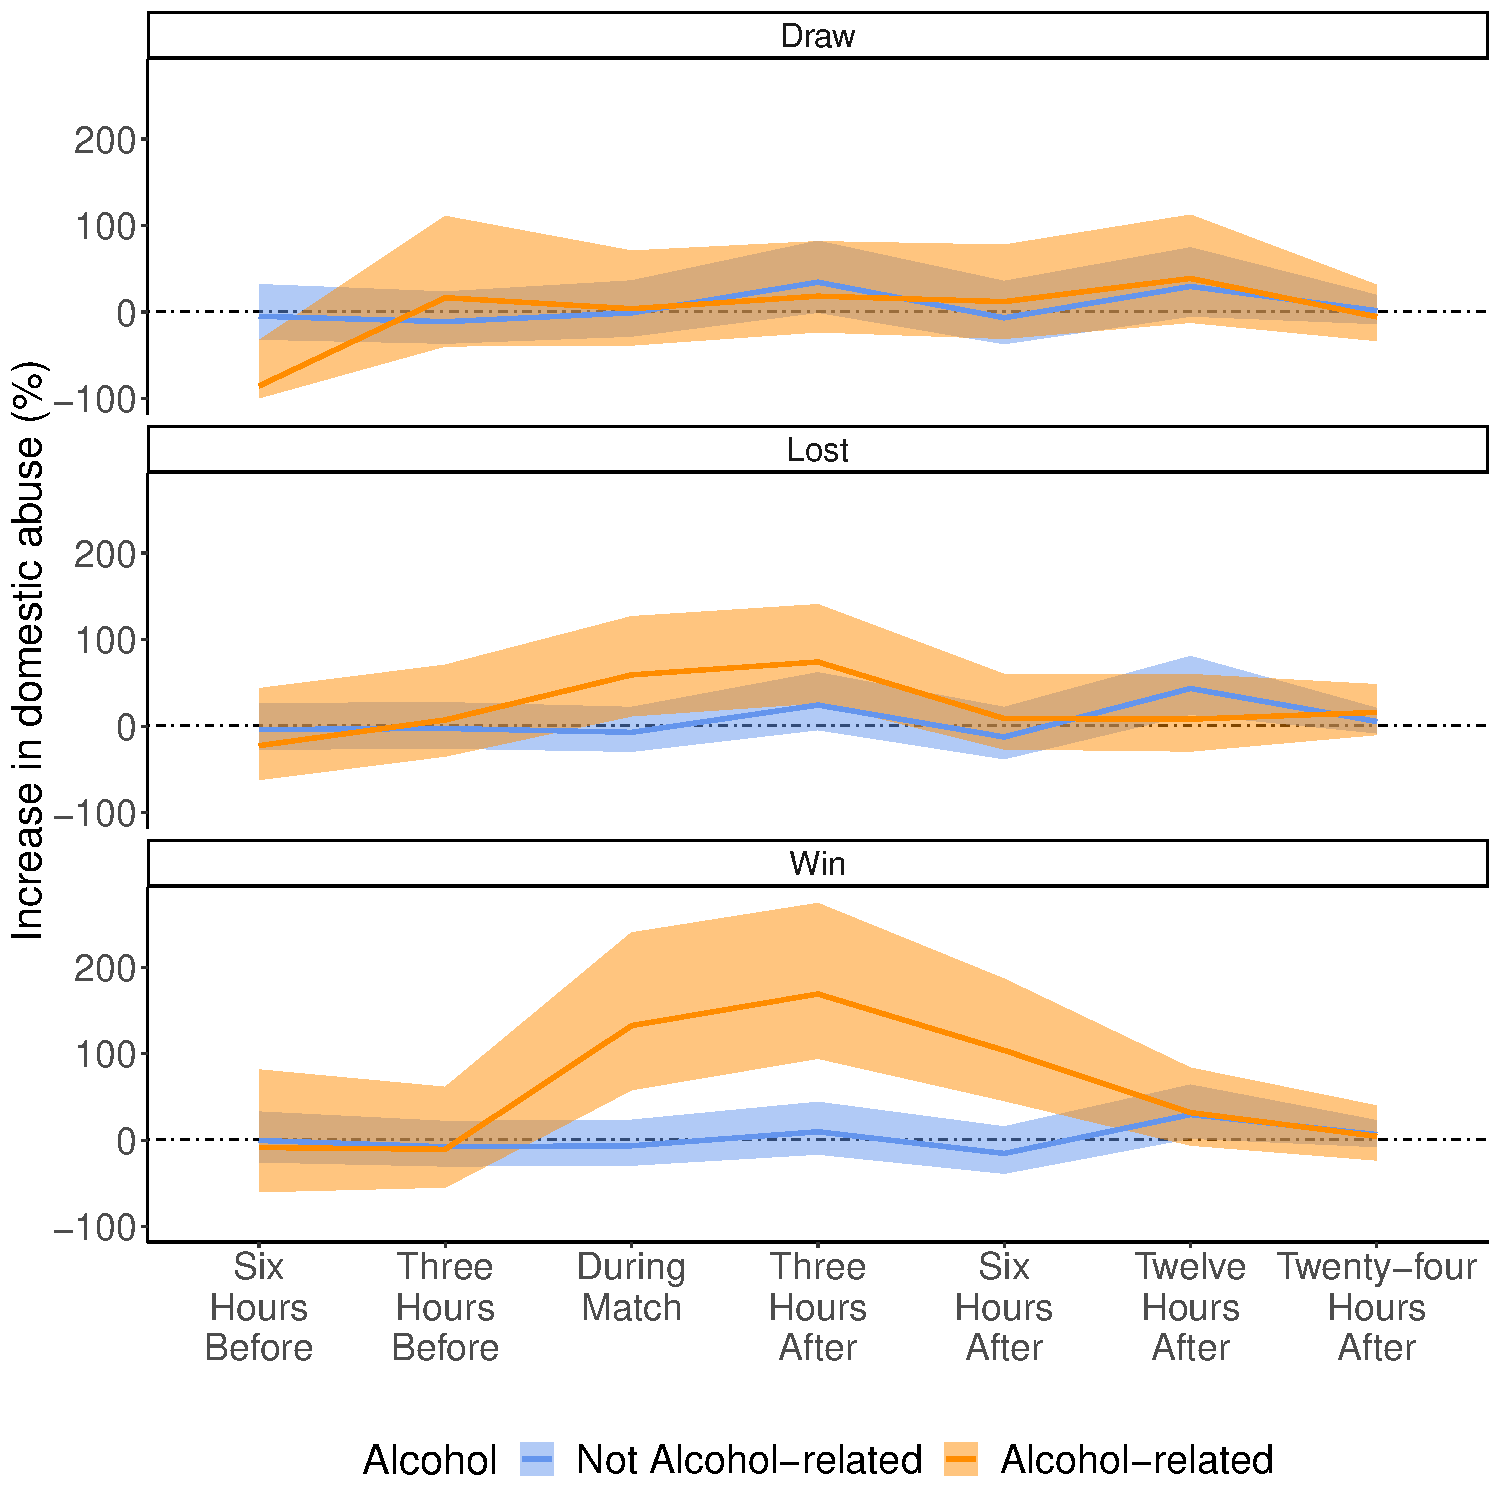
\includegraphics[width=0.75\textwidth]{Threehours.pdf}
\label{fig:threehours}
\floatfoot{Note: Estimates are from two separate negative binomial regressions (based on tests of overdispersion) with year, month, day of week, three-hour period of day, Christmas, New Year's eve controls}
\end{figure}

\newpage


\textbf{Robustness.} The increase in alcohol-related domestic abuse cases following an England victory is relatively robust to the exclusion of specific tournament years (2010, 2012, 2014, 2016), and only becomes non-significant if 2018 is excluded, because half of the England win days in our dataset comes from 2018 (see Table \ref{robustness} in the Appendix). 

\textbf{Other crimes that are about power.} We also investigated whether the number of other reported crimes that have the element of dominance \textcolor{red}{put it better}, such as sexual offences and other abuse cases (child abuse and vulnerable adult abuse) are affected by football. Table \ref{otherabuse} in the Appendix shows the results, indicating no effect for sexual offences and a similar, but less pronounced effect for alcohol-related other abuse cases on days when England wins. \textcolor{red}{sentence about sexual offences being even more underreported than DA?}

\textbf{Rugby.} It has been suggested that the relationship between football and domestic abuse in England is not unique, and that popular sports, such as rugby have similar links with domestic abuse\autocite{Brooks-Hay2018}. Focusing on the Six Nations, a high-profile rugby tournament which takes place every year, we explored whether matches of the England national rugby union team have similar effects on the reported number of domestic abuse cases. 

%The result in Table \ref{rugby} in the Appendix shows that we found no comparable effects for England matches during the Six Nations tournament. This discrepancy between the effects of rugby and football is likely to reflect the difference between the popularity and the subsequent media coverage of the two sports. 

\textcolor{red}{Table \ref{rugby2} in the appendix shows that while non-alcohol related domestic abuse decreases on days when Englands wins in the six nations, alcohol-related abuse increases. This pattern results in non-significant results when we run the regressions on the subset of alcohol-related incidents.}

\textbf{Characteristics.} To gain a deeper understanding of what drives this increase, we can analyse various characteristics of alcohol-related domestic abuse cases reported on England match days. 


% The first column in Table \ref{characteristics} in the Appendix indicate that there is no difference in the increase between alcohol-related domestic abuse incidents in public or private locations on England win days. In addition, the second column shows that when England wins, we do not see a difference between the increase in alcohol-related domestic abuse depending on whether the victim-perpetrator pair had a previous domestic abuse case reported or did not. However, given the problem of underreporting, and the serial nature of domestic abuse, we cannot be sure if newly reported cases are indeed the first occasion of abusive behaviour for that particular victim-perpetrator pair. Finally, the third column shows that alcohol-related domestic abuse happening on England win days is not more likely to result in injuries than alcohol-related domestic abuse happening on nonmatch days.   


%For example, it could be argued that the increased number of reported domestic abuse cases might be the result of a higher likelihood of the incident happening in public - the tournaments take place in the summer, and many fans choose to congregate and watch the match in a pub - although it is not immediately clear why the effect would vary by the result of the match. 


%But what kind of abuse? useful framework is the typology by Johnson (2008). Can we differentiate SCV and intimate terrorism by the time of reporting? We'd expect loads of CSV in our dataset and not much intimate terrorism (Johnson argues we should use ex partners dataset to investigate this due to the reporting bias in different types of domestic abuse). Intimate terrorism is characterised by harassment and stalking after separation. The big difference between SCV and IT is control. 


%\href{https://tavistockrelationships.ac.uk/policy-research/policy-briefings/914-couples-with-situational-violence}{Very useful classification}.


\subsection{Limitations}

It is very likely that other factors also affect the strength of the effect

underreporting, other factors like weather, campaigns may have increased willingness to report? but then why would it not be the same regardless of the result. issues about defining initimate partner violence, maybe increase because people celebrate outside? no.
If he had enough data, we could test for the same thing Card \& Lee have done.


\section{Conclusion}

context - increase in alcohol-related incidents when E wins is 62\%, NYE - 37\%, XMAS - 76\%, Friday - 28\%, Saturday - 102\%, Sunday - 94\%



\newpage

\section{Appendix}

\begin{table}[ht]
\centering
 \caption{Contrasts by alcohol and day type}
  \label{emmeans_results}
 \scalebox{0.72}{
   \begin{threeparttable}
\begin{tabular}{lrrrrl}
  \hline
contrast & estimate & SE & df & z.ratio & p.value \\ 
  \hline
\multicolumn{6}{l}{Alcohol = No}\\
Nonmatch day - Tournament on & -0.0132 & 0.0317 & Inf & -0.417 & 0.9984 \\ 
  Nonmatch day - England win & 0.0381 & 0.0972 & Inf & 0.392 & 0.9988 \\ 
  Nonmatch day - England draw & -0.0464 & 0.1116 & Inf & -0.416 & 0.9984 \\ 
  Nonmatch day - England lost & 0.0160 & 0.0952 & Inf & 0.169 & 1.0000 \\ 
  Nonmatch day - After England & -0.0701 & 0.0589 & Inf & -1.191 & 0.8416 \\ 
  Tournament on - England win & 0.0514 & 0.1007 & Inf & 0.510 & 0.9958 \\ 
  Tournament on - England draw & -0.0331 & 0.1142 & Inf & -0.290 & 0.9997 \\ 
  Tournament on - England lost & 0.0293 & 0.0986 & Inf & 0.297 & 0.9997 \\ 
  Tournament on - After England & -0.0569 & 0.0643 & Inf & -0.886 & 0.9501 \\ 
  England win - England draw & -0.0845 & 0.1465 & Inf & -0.577 & 0.9926 \\ 
  England win - England lost & -0.0221 & 0.1346 & Inf & -0.164 & 1.0000 \\ 
  England win - After England & -0.1083 & 0.1118 & Inf & -0.968 & 0.9280 \\ 
  England draw - England lost & 0.0624 & 0.1452 & Inf & 0.430 & 0.9981 \\ 
  England draw - After England & -0.0238 & 0.1243 & Inf & -0.191 & 1.0000 \\ 
  England lost - After England & -0.0862 & 0.1101 & Inf & -0.783 & 0.9705 \\ 
   \hline
\multicolumn{6}{l}{Alcohol = Yes}\\
Nonmatch day - Tournament on & 0.0544 & 0.0381 & Inf & 1.426 & 0.7111 \\ 
  Nonmatch day - England win & -0.4390 & 0.1077 & Inf & -4.078 & 0.0006 \\ 
  Nonmatch day - England draw & 0.0154 & 0.1365 & Inf & 0.113 & 1.0000 \\ 
  Nonmatch day - England lost & -0.1889 & 0.1089 & Inf & -1.734 & 0.5092 \\ 
  Nonmatch day - After England & -0.1179 & 0.0693 & Inf & -1.702 & 0.5304 \\ 
  Tournament on - England win & -0.4934 & 0.1127 & Inf & -4.376 & 0.0002 \\ 
  Tournament on - England draw & -0.0390 & 0.1403 & Inf & -0.278 & 0.9998 \\ 
  Tournament on - England lost & -0.2432 & 0.1138 & Inf & -2.136 & 0.2684 \\ 
  Tournament on - After England & -0.1723 & 0.0767 & Inf & -2.245 & 0.2172 \\ 
  England win - England draw & 0.4544 & 0.1726 & Inf & 2.632 & 0.0896 \\ 
  England win - England lost & 0.2502 & 0.1518 & Inf & 1.648 & 0.5666 \\ 
  England win - After England & 0.3211 & 0.1264 & Inf & 2.541 & 0.1124 \\ 
  England draw - England lost & -0.2042 & 0.1734 & Inf & -1.178 & 0.8475 \\ 
  England draw - After England & -0.1333 & 0.1515 & Inf & -0.880 & 0.9515 \\ 
  England lost - After England & 0.0709 & 0.1275 & Inf & 0.557 & 0.9937 \\ 
   \hline
   
%\textit{Note:}  & \multicolumn{3}{r}{Results are averaged over the levels of: year, Day_of_week, month, XMAS, NYE}    
   
%\multicolumn{6}{l}{{\footnotesize Results are averaged over the levels of: year, Day_of_week, month, XMAS, NYE}}\\

%\multicolumn{6}{l}{{\footnotesize Results are given on the log (not the response) scale.}}\\

%\multicolumn{6}{l}{{\footnotesize P value adjustment: tukey method for comparing a family of 6 estimates}}\\
\end{tabular}
\begin{tablenotes}
      \item[a] \textit{Results are from a negative binomial regression with all domestic abuse cases (see the first column of Table \ref{gender_regression})}
      \item[b] \textit{Results are averaged over the levels of: year, Day of week, month, XMAS, NYE;  Results are given on the log (not the response) scale}
    \end{tablenotes}
\end{threeparttable} }
\end{table}

\newpage

\begin{table}
\centering
 \caption{Replication of Kirby et al. (2014) and alternative specifications}
   \label{kirbyrep}
 \begin{threeparttable}
\begin{tabular}{@{\extracolsep{5pt}}lccc} 
\\[-1.8ex]\hline 
\hline \\[-1.8ex] 
 & \multicolumn{3}{c}{\textit{Dependent variable:}} \\ 
  & \multicolumn{3}{c}{Number of reported IPV cases per day} \\ 
\cline{2-4} 
\\[-1.8ex] & \multicolumn{3}{c}{} \\ 
 & Original  & Win/Draw as & Model 2 + \\ 
  &  Model & separate & month control \\ 
\\[-1.8ex] & (1) & (2) & (3)\\ 
\hline \\[-1.8ex] 
 England windraw & 0.256$^{***}$ &  &  \\ 
  & (0.055) &  &  \\ 
  England win &  & 0.452$^{***}$ & 0.458$^{***}$ \\ 
  &  & (0.064) & (0.063) \\ 
  England draw &  & 0.032 & 0.031 \\ 
  &  & (0.073) & (0.073) \\ 
  England lost & 0.382$^{***}$ & 0.388$^{***}$ & 0.326$^{***}$ \\ 
  & (0.094) & (0.085) & (0.092) \\ 
  After England & 0.111$^{**}$ & 0.113$^{**}$ & 0.101$^{**}$ \\ 
  & (0.051) & (0.047) & (0.048) \\ 
 \hline \\[-1.8ex] 
%Observations & 92 & 92 & 92 \\ 
%Log Likelihood & $-$345.490 & $-$339.178 & $-$338.439 \\ 
%$\theta$ & 80.733$^{***}$  (26.938) & 121.835$^{**}$  (53.191) & 129.150$^{**}$  (58.716) \\ 
%Akaike Inf. Crit. & 714.980 & 704.356 & 704.878 \\ 
%\hline 
%\hline \\[-1.8ex] 
%\textit{Note:}  & \multicolumn{3}{r}{$^{*}$p$<$0.1; $^{**}$p$<$0.05; $^{***}$p$<$0.01} %\\ 
\end{tabular} 
\begin{tablenotes}
      \item[a] \textit{$^{*}$p$<$0.1; $^{**}$p$<$0.05; $^{***}$p$<$0.01}
      \item[b] \textit{Estimates are from a series of negative binomial regressions  with year and day of week controls; standard errors in parentheses}
    \end{tablenotes}
\end{threeparttable} 
\end{table}

\newpage





\begin{table}
\centering
 \caption{Robustness of the result: sensitivity to the exclusion of specific years}
  \label{robustness}
 \scalebox{0.8}{
  \begin{threeparttable}
\begin{tabular}{@{\extracolsep{5pt}}lcccccc} 
\\[-1.8ex]\hline 
\hline \\[-1.8ex] 
 & \multicolumn{6}{c}{\textit{Dependent variable:}} \\ 
  & \multicolumn{6}{c}{Number of domestic abuse cases per day} \\ 
\cline{2-7} 
%\\[-1.8ex] & \multicolumn{6}{c}{DA\_incidents} \\ 
 &  All & 2018 & 2016 & 2014 & 2012 & 2010 \\ 
  & years & excluded & excluded & excluded & excluded & excluded \\ 
\\[-1.8ex] & (1) & (2) & (3) & (4) & (5) & (6)\\ 
\hline \\[-1.8ex] 
 Tournament on & 0.013 & 0.004 & 0.039 & 0.047 & 0.034 & $-$0.053 \\ 
  & (0.032) & (0.033) & (0.037) & (0.038) & (0.034) & (0.035) \\ 
  England win & $-$0.037 & $-$0.009 & $-$0.054 & $-$0.047 & 0.017 & $-$0.071 \\ 
  & (0.097) & (0.145) & (0.105) & (0.098) & (0.108) & (0.100) \\ 
  England draw & 0.047 & 0.033 & 0.149 & 0.049 & $-$0.018 & 0.043 \\ 
  & (0.112) & (0.114) & (0.139) & (0.123) & (0.120) & (0.132) \\ 
  England lost & $-$0.016 & $-$0.047 & $-$0.013 & 0.004 & 0.008 & $-$0.040 \\ 
  & (0.095) & (0.124) & (0.103) & (0.110) & (0.099) & (0.098) \\ 
  After England & 0.073 & 0.055 & 0.078 & 0.083 & 0.088 & 0.055 \\ 
  & (0.059) & (0.074) & (0.066) & (0.064) & (0.063) & (0.063) \\ 
%  Alcohol & $-$0.721$^{***}$ & $-$0.724$^{***}$ & $-$0.729$^{***}$ & $-$0.729$^{***}$ & $-$0.713$^{***}$ & $-$0.704$^{***}$ \\ 
%  & (0.008) & (0.009) & (0.009) & (0.009) & (0.008) & (0.008) \\ 
  Tournament on:Alcohol & $-$0.065 & $-$0.055 & $-$0.096$^{*}$ & $-$0.167$^{***}$ & $-$0.091$^{*}$ & 0.068 \\ 
  & (0.046) & (0.047) & (0.056) & (0.057) & (0.050) & (0.051) \\ 
  England win:Alcohol & 0.612$^{***}$ & 0.434 & 0.695$^{***}$ & 0.663$^{***}$ & 0.612$^{***}$ & 0.551$^{***}$ \\ 
  & (0.144) & (0.221) & (0.156) & (0.144) & (0.158) & (0.149) \\ 
  England draw:Alcohol & $-$0.060 & $-$0.051 & $-$0.312 & $-$0.050 & 0.064 & 0.004 \\ 
  & (0.175) & (0.177) & (0.232) & (0.193) & (0.184) & (0.204) \\ 
  England lost:Alcohol & 0.227 & 0.188 & 0.336$^{*}$ & 0.228 & 0.188 & 0.168 \\ 
  & (0.143) & (0.188) & (0.154) & (0.166) & (0.150) & (0.149) \\ 
  After England:Alcohol & 0.049 & $-$0.073 & 0.081 & 0.041 & 0.072 & 0.082 \\ 
  & (0.089) & (0.114) & (0.100) & (0.097) & (0.094) & (0.094) \\ 
 \hline \\[-1.8ex] 
Observations & 6,034 & 5,416 & 5,302 & 5,304 & 5,302 & 5,304 \\ 
%Log Likelihood & $-$23,003.430 & $-$20,532.880 & $-$20,053.510 & $-$20,101.880 & $-$20,496.330 & $-$20,250.290 \\ 
%$\theta$ & 16.979$^{***}$  (0.470) & 16.234$^{***}$  (0.473) & 16.501$^{***}$  (0.490) & 16.833$^{***}$  (0.500) & 17.570$^{***}$  (0.514) & 18.452$^{***}$  (0.550) \\ 
%Akaike Inf. Crit. & 46,084.860 & 41,141.770 & 40,183.020 & 40,279.760 & 41,068.670 & 40,576.580 \\ 
\hline 
%\hline \\[-1.8ex] 
%\textit{Note:}  & \multicolumn{6}{r}{$^{*}$p$<$0.1; $^{**}$p$<$0.05; $^{***}$p$<$0.01} \\ 
%\end{tabular} 
%\end{table} 

\end{tabular} 
\begin{tablenotes}
      \item[a] \textit{$^{*}$p$<$0.1; $^{**}$p$<$0.05; $^{***}$p$<$0.01}
      \item[b] \textit{Estimates are from a series of negative binomial regressions (based on tests of overdispersion)  with year, month, day of week, Christmas, New Year's eve controls; standard errors in parentheses}
    \end{tablenotes}
\end{threeparttable} } 
\end{table}

\newpage

\begin{table}
\centering
 \caption{Non domestic abuse incidents that are about power}
  \label{otherabuse}
  \scalebox{0.9}{
  \begin{threeparttable}
\begin{tabular}{@{\extracolsep{5pt}}lccc} 
\\[-1.8ex]\hline 
\hline \\[-1.8ex] 
 & \multicolumn{3}{c}{\textit{Dependent variable:}} \\ 
\cline{2-4} 
\\[-1.8ex] & Domestice & Sexual & Other \\ 
\\[-1.8ex] & Abuse & Offences & Abuse \\ 
\\[-1.8ex] & (1) & (2) & (3)\\ 
\hline \\[-1.8ex] 
 Tournament on & 0.013 & 0.045 & 0.009 \\ 
  & (0.032) & (0.081) & (0.046) \\ 
  England win & $-$0.037 & $-$0.143 & $-$0.138 \\ 
  & (0.097) & (0.243) & (0.138) \\ 
  England draw & 0.047 & $-$0.104 & 0.091 \\ 
  & (0.112) & (0.285) & (0.156) \\ 
  England lost & $-$0.016 & $-$0.259 & 0.058 \\ 
  & (0.095) & (0.247) & (0.138) \\ 
  After England & 0.073 & $-$0.076 & 0.029 \\ 
  & (0.059) & (0.149) & (0.084) \\ 
%  AlcoholYes & $-$0.721$^{***}$ & $-$0.895$^{***}$ & $-$0.924$^{***}$ \\ 
%  & (0.008) & (0.027) & (0.016) \\ 
  Tournament on:AlcoholYes & $-$0.065 & $-$0.038 & $-$0.002 \\ 
  & (0.046) & (0.154) & (0.090) \\ 
  England win:AlcoholYes & 0.612$^{***}$ & 0.243 & 0.622$^{*}$ \\ 
  & (0.144) & (0.465) & (0.263) \\ 
  England draw:AlcoholYes & $-$0.060 & 0.550 & 0.016 \\ 
  & (0.175) & (0.527) & (0.324) \\ 
  England lost:AlcoholYes & 0.227 & 0.639 & 0.369 \\ 
  & (0.143) & (0.452) & (0.272) \\ 
  After England:AlcoholYes & 0.049 & 0.433 & 0.016 \\ 
  & (0.089) & (0.270) & (0.174) \\ 
 \hline \\[-1.8ex] 
Observations & 6,034 & 6,034 & 6,034 \\ 
%Log Likelihood & $-$23,003.430 & $-$12,395.250 & $-$16,856.180 \\ 
%$\theta$ & 16.979$^{***}$  (0.470) & 3.037$^{***}$  (0.098) & 9.062$^{***}$  (0.326) \\ 
%Akaike Inf. Crit. & 46,084.860 & 24,868.500 & 33,790.360 \\ 
%\hline 
%\hline \\[-1.8ex] 
%\textit{Note:}  & \multicolumn{3}{r}{$^{*}$p$<$0.1; $^{**}$p$<$0.05; $^{***}$p$<$0.01} \\ 
\hline 
\end{tabular} 
\begin{tablenotes}
      \item[a] \textit{$^{*}$p$<$0.1; $^{**}$p$<$0.05; $^{***}$p$<$0.01}
      \item[b] \textit{Estimates are from a series of negative binomial regressions (based on tests of overdispersion)  with year, month, day of week, Christmas, New Year's eve controls; standard errors in parentheses}
    \end{tablenotes}
\end{threeparttable} } 
\end{table}
\newpage



\begin{table}
\centering
 \caption{Football vs Rugby}
  \label{rugby}
 \scalebox{0.75}{
\begin{tabular}{@{\extracolsep{5pt}}lcccc} 
\\[-1.8ex]\hline 
\hline \\[-1.8ex] 
% & \multicolumn{4}{c}{\textit{Dependent variable:}} \\ 
%\cline{2-5} 
\\[-1.8ex] & \multicolumn{4}{c}{N} \\ 
 & Football & Football & Rugby & Rugby \\ 
 & Alcohol & No Alcohol & Alcohol & No Alcohol \\
\\[-1.8ex] & (1) & (2) & (3) & (4)\\ 
\hline \\[-1.8ex] 
 Tournament on & $-$0.062$^{*}$ & 0.017 & $-$0.041 & 0.005 \\ 
  & (0.023) & (0.037) & (0.021) & (0.034) \\ 
  England win & 0.586$^{***}$ & $-$0.038 & 0.050 & 0.0005 \\ 
  & (0.068) & (0.096) & (0.038) & (0.057) \\ 
  England draw & $-$0.004 & 0.043 &  &  \\ 
  & (0.078) & (0.126) &  &  \\ 
  England lost & 0.147 & 0.045 & $-$0.023 & 0.057 \\ 
  & (0.066) & (0.097) & (0.059) & (0.088) \\ 
  After England & 0.122$^{*}$ & 0.079$^{*}$ & $-$0.031 & $-$0.012 \\ 
  & (0.041) & (0.064) & (0.034) & (0.053) \\ 
 \hline \\[-1.8ex] 
%Observations & 3,017 & 3,017 & 3,017 & 3,017 \\ 
%Log Likelihood & $-$11,990.480 & $-$9,418.851 & $-$11,992.170 & $-$9,432.978 \\ 
%$\theta$ & 45.611$^{***}$  (1.902) & 26.230$^{***}$  (1.526) & 45.524$^{***}$  (1.897) & 25.712$^{***}$  (1.482) \\ 
%Akaike Inf. Crit. & 24,046.970 & 18,903.700 & 24,048.350 & 18,929.960 \\ 
%\hline 
%\hline \\[-1.8ex] 
%\textit{Note:}  & \multicolumn{4}{r}{$^{*}$p$<$0.1; $^{**}$p$<$0.05; $^{***}$p$<$0.01} \\ 
\end{tabular} }
\end{table}


\begin{table}
\centering
 \caption{Football vs Rugby2}
  \label{rugby2}
 \scalebox{0.75}{
\begin{tabular}{@{\extracolsep{5pt}}lcc} 
\\[-1.8ex]\hline 
\hline \\[-1.8ex] 
 & \multicolumn{2}{c}{\textit{Dependent variable:}} \\ 
\cline{2-3} 
\\[-1.8ex] & \multicolumn{2}{c}{Domestic\_Abuse} \\ 
\\[-1.8ex] & (1) & (2)\\ 
\hline \\[-1.8ex] 
 Tournament on & 0.013 & 0.037 \\ 
  & (0.032) & (0.025) \\ 
  England win & $-$0.037 & $-$0.138$^{***}$ \\ 
  & (0.097) & (0.052) \\ 
  England draw & 0.047 &  \\ 
  & (0.112) &  \\ 
  England lost & $-$0.016 & $-$0.095 \\ 
  & (0.095) & (0.083) \\ 
  After England & 0.073 & $-$0.083$^{*}$ \\ 
  & (0.059) & (0.045) \\ 
  Alcohol & $-$0.721$^{***}$ & $-$0.719$^{***}$ \\ 
  & (0.008) & (0.008) \\ 
  Tournament on:Alcohol & $-$0.065 & $-$0.123$^{***}$ \\ 
  & (0.046) & (0.026) \\ 
  England win:Alcohol & 0.612$^{***}$ & 0.453$^{***}$ \\ 
  & (0.144) & (0.071) \\ 
  England draw:Alcohol & $-$0.060 &  \\ 
  & (0.175) &  \\ 
  England lost:Alcohol & 0.227 & 0.273$^{*}$ \\ 
  & (0.143) & (0.123) \\ 
  After England:Alcohol & 0.049 & 0.154$^{**}$ \\ 
  & (0.089) & (0.062) \\ 
 \hline \\[-1.8ex] 
Observations & 6,034 & 6,034 \\ 
Log Likelihood & $-$23,003.430 & $-$22,984.260 \\ 
$\theta$ & 16.979$^{***}$  (0.470) & 17.171$^{***}$  (0.477) \\ 
Akaike Inf. Crit. & 46,084.860 & 46,042.530 \\ 
\hline 
\hline \\[-1.8ex] 
\textit{Note:}  & \multicolumn{2}{r}{$^{*}$p$<$0.1; $^{**}$p$<$0.05; $^{***}$p$<$0.01} \\ 
\end{tabular}  }
\end{table}




\newpage

\begin{table}
\centering
 \caption{Characteristics of alcohol-related domestic abuse cases}
 \scalebox{0.75}{
 \label{characteristics}
\begin{tabular}{@{\extracolsep{5pt}}lcccccc} 
\\[-1.8ex]\hline 
\hline \\[-1.8ex] 
 & \multicolumn{6}{c}{\textit{Dependent variable:}} \\ 
\cline{2-7} 
\\[-1.8ex] & \multicolumn{6}{c}{N} \\ 
\\[-1.8ex] & Alcohol & No Alcohol & Alcohol & No Alcohol & Alcohol & No Alcohol\\ 
\\[-1.8ex] & (1) & (2) & (3) & (4) & (5) & (6)\\ 
\hline \\[-1.8ex] 
 Tournament on & $-$0.077$^{**}$ & 0.008 & $-$0.095$^{*}$ & 0.034 & $-$0.060 & 0.010 \\ 
  & (0.038) & (0.024) & (0.055) & (0.035) & (0.040) & (0.025) \\ 
  England win & 0.484$^{***}$ & $-$0.084 & 0.432$^{**}$ & 0.007 & 0.385$^{***}$ & $-$0.064 \\ 
  & (0.101) & (0.073) & (0.139) & (0.101) & (0.108) & (0.077) \\ 
  England draw & $-$0.016 & 0.033 & 0.131 & 0.046 & $-$0.009 & 0.005 \\ 
  & (0.132) & (0.083) & (0.198) & (0.133) & (0.140) & (0.089) \\ 
  England lost & 0.060 & $-$0.025 & 0.023 & 0.121 & 0.158 & $-$0.010 \\ 
  & (0.103) & (0.071) & (0.146) & (0.097) & (0.107) & (0.075) \\ 
  After England & 0.083 & 0.048 & 0.167$^{*}$ & 0.103$^{*}$ & 0.100 & 0.065 \\ 
  & (0.067) & (0.044) & (0.092) & (0.062) & (0.071) & (0.046) \\ 
  Locationpublic & $-$0.871$^{***}$ & $-$0.850$^{***}$ &  &  &  &  \\ 
  & (0.014) & (0.008) &  &  &  &  \\ 
  Newlyreported &  &  & 0.488$^{***}$ & 0.610$^{***}$ &  &  \\ 
  &  &  & (0.011) & (0.007) &  &  \\ 
  Serious &  &  &  &  & $-$1.129$^{***}$ & $-$1.514$^{***}$ \\ 
  &  &  &  &  & (0.011) & (0.007) \\ 
  Tournament on:Locationpublic & 0.115 & 0.048 &  &  &  &  \\ 
  & (0.079) & (0.044) &  &  &  &  \\ 
  England win:Locationpublic & 0.514$^{**}$ & 0.336$^{**}$ &  &  &  &  \\ 
  & (0.191) & (0.135) &  &  &  &  \\ 
  England draw:Locationpublic & 0.077 & 0.058 &  &  &  &  \\ 
  & (0.297) & (0.164) &  &  &  &  \\ 
  England lost:Locationpublic & 0.638$^{**}$ & 0.511$^{***}$ &  &  &  &  \\ 
  & (0.197) & (0.126) &  &  &  &  \\ 
  After England:Locationpublic & 0.261$^{*}$ & 0.168$^{*}$ &  &  &  &  \\ 
  & (0.136) & (0.081) &  &  &  &  \\ 
  Tournament on:Newlyreported &  &  & 0.076 & $-$0.055 &  &  \\ 
  &  &  & (0.069) & (0.045) &  &  \\ 
  England win:Newlyreported &  &  & $-$0.006 & $-$0.101 &  &  \\ 
  &  &  & (0.187) & (0.134) &  &  \\ 
  England draw:Newlyreported &  &  & $-$0.186 & $-$0.016 &  &  \\ 
  &  &  & (0.271) & (0.176) &  &  \\ 
  England lost:Newlyreported &  &  & 0.062 & $-$0.167 &  &  \\ 
  &  &  & (0.193) & (0.130) &  &  \\ 
  After England:Newlyreported &  &  & $-$0.078 & $-$0.069 &  &  \\ 
  &  &  & (0.123) & (0.082) &  &  \\ 
  Tournament on:Serious &  &  &  &  & $-$0.032 & 0.034 \\ 
  &  &  &  &  & (0.066) & (0.041) \\ 
  England win:Serious &  &  &  &  & 0.235 & 0.162 \\ 
  &  &  &  &  & (0.173) & (0.133) \\ 
  England draw:Serious &  &  &  &  & 0.015 & 0.182 \\ 
  &  &  &  &  & (0.244) & (0.151) \\ 
  England lost:Serious &  &  &  &  & $-$0.094 & 0.283$^{**}$ \\ 
  &  &  &  &  & (0.187) & (0.125) \\ 
  After England:Serious &  &  &  &  & 0.033 & 0.064 \\ 
  &  &  &  &  & (0.118) & (0.079) \\ 
 \hline \\[-1.8ex] 
Observations & 6,034 & 6,034 & 5,304 & 5,304 & 6,034 & 6,034 \\ 
%Log Likelihood & $-$14,525.790 & $-$19,697.630 & $-$14,611.100 & $-$18,765.770 & $-$15,726.150 & $-$20,444.700 \\ 
%$\theta$ & 24.648$^{***}$  (1.454) & 40.035$^{***}$  (1.605) & 17.346$^{***}$  (0.856) & 29.566$^{***}$  (1.045) & 22.018$^{***}$  (1.249) & 34.613$^{***}$  (1.351) \\ 
%Akaike Inf. Crit. & 29,129.580 & 39,473.260 & 29,298.200 & 37,607.550 & 31,530.290 & 40,967.400 \\ 
\hline 
\hline \\[-1.8ex] 
\textit{Note:}  & \multicolumn{6}{r}{$^{*}$p$<$0.1; $^{**}$p$<$0.05; $^{***}$p$<$0.01} \\ 
\end{tabular} }
\end{table}

\newpage

\begin{table}
\centering
 \caption{Alcohol transition}
 \scalebox{0.75}{
\begin{tabular}{@{\extracolsep{5pt}}lc} 
\\[-1.8ex]\hline 
\hline \\[-1.8ex] 
 & \multicolumn{1}{c}{\textit{Dependent variable:}} \\ 
\cline{2-2} 
\\[-1.8ex] & Alcohol \\ 
\hline \\[-1.8ex] 
 TypeTournament\_on & $-$0.137$^{**}$ \\ 
  & (0.067) \\ 
  TypeEngland\_win & 0.548$^{***}$ \\ 
  & (0.156) \\ 
  TypeEngland\_draw & 0.460$^{*}$ \\ 
  & (0.202) \\ 
  TypeEngland\_lost & $-$0.105 \\ 
  & (0.177) \\ 
  TypeAfter\_England & 0.035 \\ 
  & (0.112) \\ 
  Previous\_alcYes & 5.196$^{***}$ \\ 
  & (0.017) \\ 
  TypeTournament\_on:Previous\_alcYes & $-$0.055 \\ 
  & (0.098) \\ 
  TypeEngland\_win:Previous\_alcYes & $-$0.082 \\ 
  & (0.265) \\ 
  TypeEngland\_draw:Previous\_alcYes & $-$0.306 \\ 
  & (0.375) \\ 
  TypeEngland\_lost:Previous\_alcYes & 0.209 \\ 
  & (0.279) \\ 
  TypeAfter\_England:Previous\_alcYes & 0.094 \\ 
  & (0.172) \\ 
 \hline \\[-1.8ex] 
Observations & 97,292 \\ 
Log Likelihood & $-$48,223.270 \\ 
Akaike Inf. Crit. & 96,524.550 \\ 
\hline 
\hline \\[-1.8ex] 
\textit{Note:}  & \multicolumn{1}{r}{$^{*}$p$<$0.1; $^{**}$p$<$0.05; $^{***}$p$<$0.01} \\ 
\end{tabular} 
}
\end{table}
\newpage

\begin{table}
\centering
 \caption{}
 \scalebox{0.75}{
\begin{tabular}{@{\extracolsep{5pt}}lccc} 
\\[-1.8ex]\hline 
\hline \\[-1.8ex] 
 & \multicolumn{3}{c}{\textit{Dependent variable:}} \\ 
\cline{2-4} 
\\[-1.8ex] & Daystilnext\_round & Dayssincelast\_round & Report\_delay \\ 
\\[-1.8ex] & (1) & (2) & (3)\\ 
\hline \\[-1.8ex] 
 TypeTournament\_on & $-$0.022 & 0.028 & 0.002 \\ 
  & (0.030) & (0.032) & (0.049) \\ 
  TypeEngland\_win & $-$0.212$^{**}$ & 0.127 & $-$0.518$^{***}$ \\ 
  & (0.106) & (0.090) & (0.144) \\ 
  TypeEngland\_draw & 0.061 & 0.005 & $-$0.525$^{***}$ \\ 
  & (0.104) & (0.117) & (0.168) \\ 
  TypeEngland\_lost & $-$0.124 & $-$0.089 & $-$0.559$^{***}$ \\ 
  & (0.095) & (0.085) & (0.137) \\ 
  TypeAfter\_England & $-$0.064 & 0.067 & $-$0.516$^{***}$ \\ 
  & (0.058) & (0.055) & (0.085) \\ 
  AlcoholYes & $-$0.028$^{***}$ & 0.029$^{***}$ & $-$0.784$^{***}$ \\ 
  & (0.010) & (0.010) & (0.017) \\ 
  TypeTournament\_on:AlcoholYes & 0.053 & 0.011 & $-$0.014 \\ 
  & (0.055) & (0.060) & (0.095) \\ 
  TypeEngland\_win:AlcoholYes & 0.174 & 0.030 & 1.867$^{***}$ \\ 
  & (0.188) & (0.154) & (0.251) \\ 
  TypeEngland\_draw:AlcoholYes & $-$0.305$^{*}$ & $-$0.166 & $-$0.618$^{*}$ \\ 
  & (0.202) & (0.213) & (0.351) \\ 
  TypeEngland\_lost:AlcoholYes & 0.086 & 0.244 & $-$0.142 \\ 
  & (0.174) & (0.166) & (0.266) \\ 
  TypeAfter\_England:AlcoholYes & 0.062 & 0.008 & 0.160 \\ 
  & (0.113) & (0.103) & (0.169) \\ 
 \hline \\[-1.8ex] 
Observations & 97,292 & 97,292 & 277,753 \\ 
Log Likelihood & $-$620,751.900 & $-$623,803.700 & $-$702,611.400 \\ 
$\theta$ & 0.583$^{***}$  (0.002) & 0.556$^{***}$  (0.002) & 0.079$^{***}$  (0.0002) \\ 
Akaike Inf. Crit. & 1,241,582.000 & 1,247,685.000 & 1,405,301.000 \\ 
\hline 
\hline \\[-1.8ex] 
\textit{Note:}  & \multicolumn{3}{r}{$^{*}$p$<$0.1; $^{**}$p$<$0.05; $^{***}$p$<$0.01} \\ 
\end{tabular}}
\end{table}

\newpage

\begin{table}
\centering
 \caption{}
 \scalebox{0.75}{
\begin{tabular}{@{\extracolsep{5pt}}lcccc} 
\\[-1.8ex]\hline 
\hline \\[-1.8ex] 
 & \multicolumn{4}{c}{\textit{Dependent variable:}} \\ 
\cline{2-5} 
\\[-1.8ex] & \multicolumn{4}{c}{Income\_no} \\ 
\\[-1.8ex] & Lowest & Lower & Higher & Highest\\ 
\\[-1.8ex] & (1) & (2) & (3) & (4)\\ 
\hline \\[-1.8ex] 
 Type.of.dayTournament on & 0.018 & $-$0.022 & 0.121$^{*}$ & $-$0.038 \\ 
  & (0.033) & (0.045) & (0.062) & (0.093) \\ 
  Type.of.dayEngland win & $-$0.070 & $-$0.065 & 0.172 & $-$0.482$^{*}$ \\ 
  & (0.102) & (0.136) & (0.183) & (0.344) \\ 
  Type.of.dayEngland draw & 0.119 & $-$0.085 & $-$0.181 & $-$0.137 \\ 
  & (0.115) & (0.161) & (0.246) & (0.339) \\ 
  Type.of.dayEngland lost & $-$0.081 & $-$0.107 & 0.365$^{*}$ & 0.050 \\ 
  & (0.099) & (0.134) & (0.166) & (0.252) \\ 
  Type.of.dayAfter England & 0.103 & 0.006 & 0.100 & $-$0.137 \\ 
  & (0.061) & (0.082) & (0.114) & (0.173) \\ 
  AlcoholYes & $-$0.718$^{***}$ & $-$0.685$^{***}$ & $-$0.681$^{***}$ & $-$0.706$^{***}$ \\ 
  & (0.009) & (0.013) & (0.019) & (0.029) \\ 
  Type.of.dayTournament on:AlcoholYes & $-$0.073 & $-$0.022 & $-$0.104 & 0.129 \\ 
  & (0.050) & (0.076) & (0.110) & (0.161) \\ 
  Type.of.dayEngland win:AlcoholYes & 0.585$^{***}$ & 0.639$^{**}$ & $-$0.053 & 2.795$^{***}$ \\ 
  & (0.154) & (0.216) & (0.345) & (0.473) \\ 
  Type.of.dayEngland draw:AlcoholYes & $-$0.187 & 0.355 & 0.327 & $-$0.069 \\ 
  & (0.191) & (0.268) & (0.427) & (0.684) \\ 
  Type.of.dayEngland lost:AlcoholYes & 0.255 & 0.290 & $-$0.146 & $-$0.192 \\ 
  & (0.154) & (0.225) & (0.320) & (0.525) \\ 
  Type.of.dayAfter England:AlcoholYes & $-$0.034 & 0.080 & 0.235 & 0.562 \\ 
  & (0.096) & (0.140) & (0.195) & (0.288) \\ 
 \hline \\[-1.8ex] 
Observations & 6,034 & 6,034 & 6,034 & 6,034 \\ 
Log Likelihood & $-$20,792.850 & $-$14,570.920 & $-$11,316.060 & $-$8,282.382 \\ 
$\theta$ & 17.652$^{***}$  (0.568) & 18.443$^{***}$  (1.181) & 14.978$^{***}$  (1.533) & 8.905$^{***}$  (1.200) \\ 
Akaike Inf. Crit. & 41,663.700 & 29,219.840 & 22,710.130 & 16,642.760 \\ 
\hline 
\hline \\[-1.8ex] 
\textit{Note:}  & \multicolumn{4}{r}{$^{*}$p$<$0.1; $^{**}$p$<$0.05; $^{***}$p$<$0.01} \\ 
\end{tabular} }
\end{table}

\newpage

\begin{table}
\centering
 \caption{Deprivation}
 \scalebox{0.75}{
 \begin{tabular}{@{\extracolsep{5pt}}lcccc} 
\\[-1.8ex]\hline 
\hline \\[-1.8ex] 
 & \multicolumn{4}{c}{\textit{Dependent variable:}} \\ 
\cline{2-5} 
\\[-1.8ex] & \multicolumn{4}{c}{Employment\_no} \\ 
\\[-1.8ex] & Lowest & Lower & Higher & Highest\\ 
\\[-1.8ex] & (1) & (2) & (3) & (4)\\ 
\hline \\[-1.8ex] 
 Type.of.dayTournament on & 0.018 & $-$0.002 & 0.066 & $-$0.049 \\ 
  & (0.033) & (0.045) & (0.061) & (0.095) \\ 
  Type.of.dayEngland win & $-$0.084 & 0.023 & $-$0.021 & $-$0.355 \\ 
  & (0.102) & (0.133) & (0.188) & (0.314) \\ 
  Type.of.dayEngland draw & 0.145 & $-$0.191 & $-$0.315 & 0.463 \\ 
  & (0.114) & (0.166) & (0.252) & (0.280) \\ 
  Type.of.dayEngland lost & $-$0.085 & $-$0.018 & 0.115 & 0.075 \\ 
  & (0.099) & (0.130) & (0.172) & (0.248) \\ 
  Type.of.dayAfter England & 0.109$^{*}$ & $-$0.013 & 0.045 & $-$0.068 \\ 
  & (0.061) & (0.082) & (0.112) & (0.168) \\ 
  AlcoholYes & $-$0.716$^{***}$ & $-$0.695$^{***}$ & $-$0.686$^{***}$ & $-$0.698$^{***}$ \\ 
  & (0.009) & (0.013) & (0.019) & (0.029) \\ 
  Type.of.dayTournament on:AlcoholYes & $-$0.058 & $-$0.043 & $-$0.161 & 0.121 \\ 
  & (0.050) & (0.075) & (0.111) & (0.165) \\ 
  Type.of.dayEngland win:AlcoholYes & 0.603$^{***}$ & 0.425 & 0.797$^{**}$ & 0.687 \\ 
  & (0.154) & (0.218) & (0.297) & (0.524) \\ 
  Type.of.dayEngland draw:AlcoholYes & $-$0.294$^{*}$ & 0.845$^{**}$ & 1.194$^{**}$ & $-$0.610 \\ 
  & (0.195) & (0.259) & (0.383) & (0.768) \\ 
  Type.of.dayEngland lost:AlcoholYes & 0.247 & 0.128 & 0.265 & $-$0.367 \\ 
  & (0.155) & (0.225) & (0.297) & (0.566) \\ 
  Type.of.dayAfter England:AlcoholYes & $-$0.040 & 0.143 & 0.248 & 0.354 \\ 
  & (0.096) & (0.140) & (0.190) & (0.292) \\ 
 \hline \\[-1.8ex] 
Observations & 6,034 & 6,034 & 6,034 & 6,034 \\ 
Log Likelihood & $-$20,726.560 & $-$14,694.740 & $-$11,574.920 & $-$7,884.137 \\ 
$\theta$ & 17.768$^{***}$  (0.575) & 17.855$^{***}$  (1.105) & 14.521$^{***}$  (1.359) & 11.281$^{***}$  (1.878) \\ 
Akaike Inf. Crit. & 41,531.130 & 29,467.490 & 23,227.840 & 15,846.270 \\ 
\hline 
\hline \\[-1.8ex] 
\textit{Note:}  & \multicolumn{4}{r}{$^{*}$p$<$0.1; $^{**}$p$<$0.05; $^{***}$p$<$0.01} \\ 
\end{tabular} 
 
  }
\end{table}

\clearpage
\printbibliography
\end{document}
